% "Станет проще"

\documentclass[a4paper,12pt]{article} % тип документа

% report, book

%  Русский язык

\usepackage[T2A]{fontenc}			% кодировка
\usepackage[utf8]{inputenc}			% кодировка исходного текста
\usepackage{graphicx}
\usepackage[english,russian]{babel}	% локализация и переносы


%отступ
\usepackage[left=3cm,right=3cm,
    top=3cm,bottom=3cm,bindingoffset=0cm]{geometry}

% Математика
\usepackage{amsmath,amsfonts,amssymb,amsthm,mathtools} 
\usepackage{csvsimple}
\usepackage{multirow}

\usepackage{hyperref}
\usepackage{wasysym}
\usepackage{subcaption}
\usepackage{verbatim}
\usepackage{hyperref}
\usepackage{float}
\usepackage{enumerate}
\usepackage[dvipsnames]{xcolor}
%Заговолок
%\graphicspath{ {images/} }


\begin{titlepage}
\author{Соловьянов Михаил }
\title{Задание 5. Электродинамика.  Цепи с конденсаторами}
\date{\today}
\end{titlepage}



\begin{document} % начало документа
\maketitle



\begin{figure}[H]
  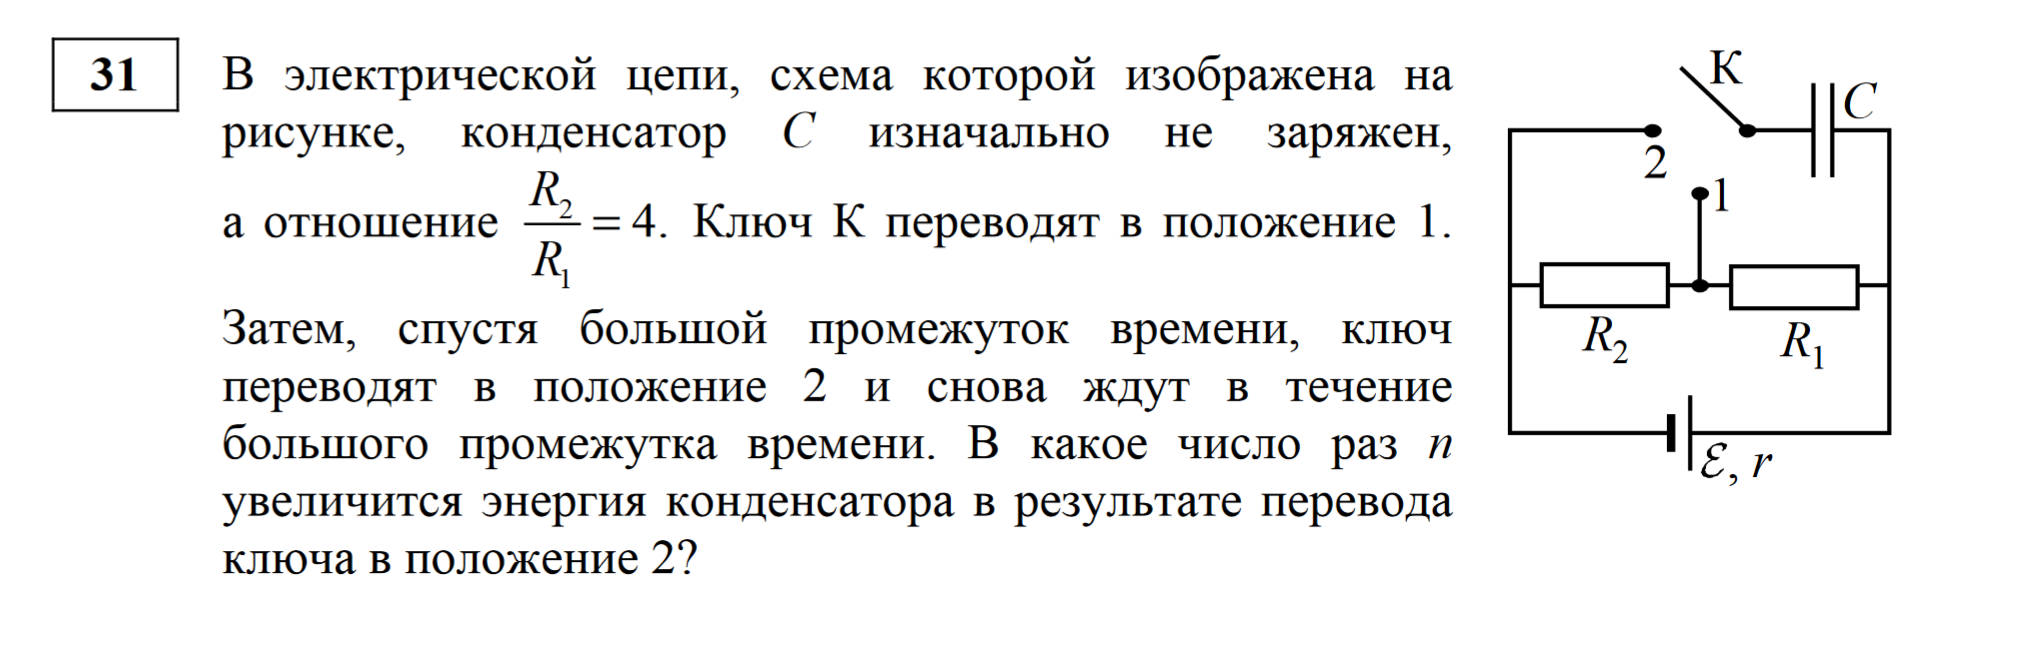
\includegraphics[width=\linewidth]{1.PNG}
  \caption{Задача 4 }
  \label{task1}
\end{figure}
 
 
 
\begin{figure}[H]
  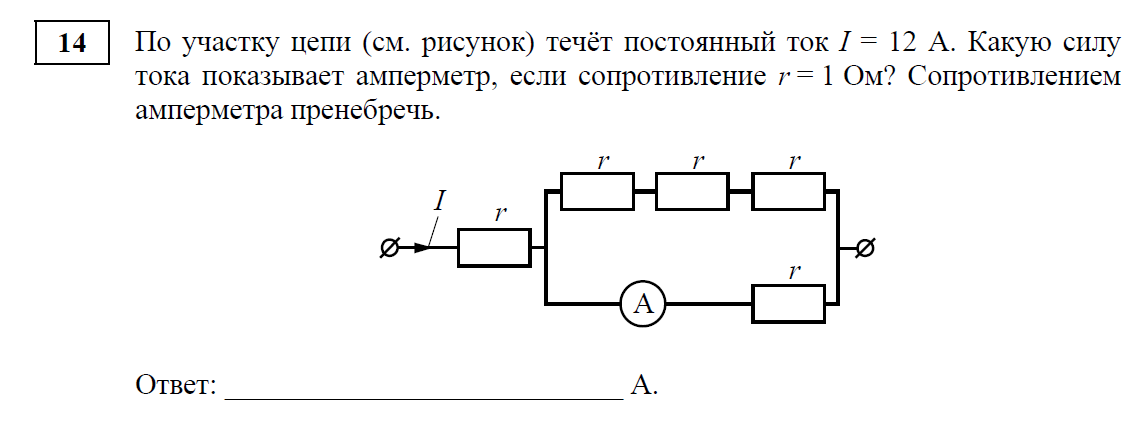
\includegraphics[width=\linewidth]{2.PNG}
  \caption{Задача 5 }
  \label{task2}
\end{figure}





\section{Контрольные вопросы}
\begin{enumerate}

\item Что называется зарядом конденсатора?  \colorbox{BrickRed}{+++++}
\item Конденсатор подключён в электрическую цепь. При каком условии напряжение на конденсаторе меняется плавно? (Если не получиться ответить разберем) \colorbox{BrickRed}{+++++}
\end{enumerate}


\section{Задачи}
\begin{enumerate}
\item Задача 3.22 \cite{l1} \colorbox{BrickRed}{Дорешать исправив очепятку}

\item  Задача 6 из \cite{l2}  \colorbox{BrickRed}{Напряжение найдено правильно, найти теперь ток правильно!}

\item  Задача 8 из \cite{l2}  \colorbox{BrickRed}{разберем пришлю похожую}

\item Задача на рисунке \ref{task1} \colorbox{BrickRed}{+++++}

\item Задача на рисунке \ref{task2} \colorbox{BrickRed}{+++++}


\item[$\ast$] Задача 7 из \cite{l2}

\end{enumerate}

\section{Литература}
\begin{thebibliography}{}
    \bibitem{l1} СБОРНИК ОЛИМПИАДНЫХ ЗАДАЧ ПО ФИЗИКЕ Под редакцией Н.С. Кравченко
    \bibitem{l2} \url{https://vk.com/doc87612555_527254723?hash=54b73288a84f13bd56&dl=e2abb02099a4d83d46}
	
\end{thebibliography}



\end{document}